\chapter{Návrh systému} \label{cha:proposed-system}

V~rámci tejto kapitoly popíšeme návrh systému určeného na automatickú detekciu nesprávnej výslovnosti. Systém je do veľkej miery inšpirovaný prácou \cite{Arora2017}, aby sme si mohli overiť a porovnať nami dosiahnuté výsledky. Všetky použité metódy a algoritmy boli popísané v~kapitolách \ref{cha:asr-systems} -- \ref{cha:mispronunciation-evaluation}.

\section{Časti systému}

Systém pozostáva z~niekoľkých častí, ktoré sú schematicky znázornené na obr. \ref{fig:system-design}. 
Nakoľko v~rámci experimentov budeme testovať niekoľko odlišných prístupov, schéma je do veľkej miery abstraktná, aby postihla všetky tieto varianty.
Dôležitou časťou celého systému je akustický model, ktorý realizuje zarovnanie reči podľa kanonického prepisu. Ďalšou podstatnou súčasťou sú príznaky, pričom ich typ závisí na použitej metóde detekcie. V~prípade GOP metódy sú nimi vierohodnosti jednotlivých HMM stavov. Získanie týchto príznakov zabezpečuje neurónová sieť, ktorá je zároveň súčasťou DNN-HMM akustického modelu. Pri hodnotení výslovnosti pomocou klasifikátora je možné použiť celú radu príznakov. V~našej práci využijeme dva typy, a to jednak už spomínané vierohodnosti HMM stavov, ale taktiež pravdepodobnosti fonologických rysov určené samostatne natrénovanou neurónovou sieťou.

\begin{figure}
    \centering
    \newif\ifstandalone
\standalonetrue % comment out for compilation with ktikz

\ifstandalone
\documentclass{standalone}
\fi

\usetikzlibrary{shapes.geometric, arrows, positioning, arrows.meta, calc}

\def\xconnection (#1,#2) {\draw[connection] (#1.north west) -- (#2.south east);  \draw[connection] (#1.north east) -- (#2.south west);}
\def\connection (#1,#2) {\draw[connection] (#1.north west) -- (#2.south west);  \draw[connection] (#1.north east) -- (#2.south east);}

\ifstandalone
\begin{document}
\fi

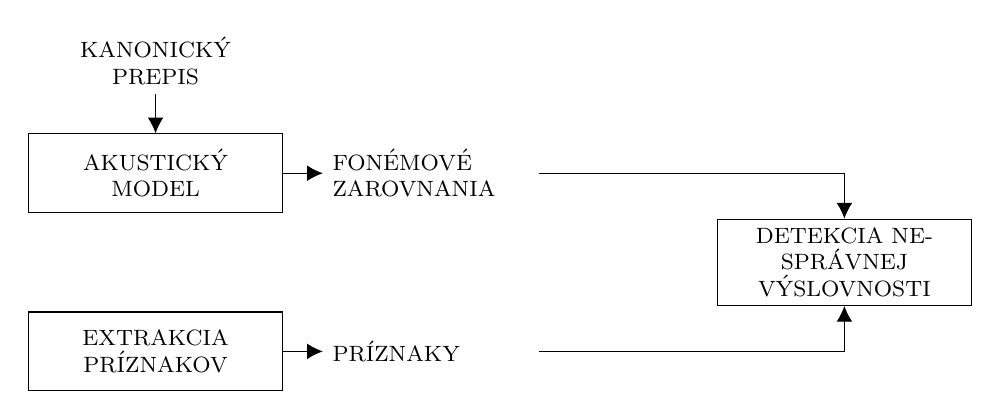
\begin{tikzpicture}[every node/.style = {font=\footnotesize}, node distance=2cm, >={Latex[width=2mm,length=2mm]}]
		\tikzstyle{punkt} = [rectangle, rounded corners, draw=black, very thick, text width=6.5em, minimum height=2em, text centered]
		\tikzstyle{pil} = [->,thick,shorten <= 2pt, shorten >= 2pt]
		\tikzstyle{block} = [rectangle, minimum width=3cm, minimum height=1cm, text centered, text width=3cm, draw=black]
		\tikzstyle{io} = [text width=2.5cm, align=flush left]
		% \tikzstyle{arrow} = [thick,->,>=stealth]
		\tikzstyle{arrow} = [->]

	    \node[block] (am) {AKUSTICKÝ MODEL};
        \node[io, text centered, above=0.5cm of am] (am-input) {KANONICKÝ PREPIS};
        \node[io, right=0.5cm of am] (am-output) {FONÉMOVÉ ZAROVNANIA};
        \node[below=0.5cm of am] (dummy) {};
        \node[block, below=0.5cm of dummy] (fe) {EXTRAKCIA PRÍZNAKOV};
        \node[io, right=0.5cm of fe] (fe-output) {PRÍZNAKY};
        \node[block, right=7cm of dummy] (md) {DETEKCIA NESPRÁVNEJ VÝSLOVNOSTI};
        \draw[arrow] (am) -- (am-output);
        \draw[arrow] (am-input) -- (am);
        \draw[arrow] (am-output) -| (md);
        \draw[arrow] (fe) -- (fe-output);
        \draw[arrow] (fe-output) -| (md);
\end{tikzpicture}

\ifstandalone
\end{document}
\fi
    \caption{Schematické znázornenie systému pre detekciu nesprávnej výslovnosti.}
    \label{fig:system-design}
\end{figure}


\section{Akustický model}

Pre modelovanie reči využijeme HMM v~kombinácii s~hlbokou neurónovou sieťou (\textit{Deep Neural Network}, DNN). Akustický model v~systéme bude slúžiť na získanie fonémových zarovnaní a extrakciu príznakov z~nenatívnej reči. Z~tohto dôvodu musí byť aj trénovaný nad nenatívnym datasetom, konkrétne nad skutočnými fonémovými prepismi.

Jednotlivé fonémy budeme reprezentovať jednak nezávisle (monofónový model), ale aj ako kontextovo závislé na susedných fonémach (trifónový model). Modely foném v~oboch prípadoch pozostávajú z~troch stavov, tak ako na obr. \ref{fig:hmm-phone}. Rovnaký počet stavov, len s~dodatočnými prechodmi (viď obr. \ref{fig:hmm-sil}), bude použitý aj pri modelovaní ticha.

Pred samotným trénovaním DNN je potrebné zarovnať trénovacie dáta pomocou skôr natrénovaného GMM-HMM modelu. V~prípade GMM sú vstupom modelu MFCC príznaky. Napriek tomu, že tieto príznaky by bolo možné použiť aj v~prípade trénovania DNN, vhodnejšie je použitie filter bank (označované aj fbank) príznakov, nakoľko u~nich bývajú dosahované lepšie výsledky \cite{Mohamed2012}. 
Pre dosiahnutie dobrej konvergencie neurónovej siete je však nevyhnutná ich normalizácia na nulovú strednú hodnotu a jednotkový rozptyl. Okrem toho zahrnieme do príznakového vektora odpovedajúceho nejakému rámcu aj hodnoty pre istý počet okolitých rámcov, vďaka čomu získa neurónová sieť určitú informáciu o~kontexte.

\subsection*{Multilingválne akustické modely}

V~rámci našich experimentov budeme skúmať, aký má vplyv použitie DNN-HMM akustického modelu natrénovaného na viacerých jazykoch. Presnejšie povedané, na viacerých jazykoch je trénovaná len DNN a HMM pochádza z~GMM-HMM modelu natrénovaného len na príslušnom jazyku. Predpokladáme totiž, že keďže je nenatívny dataset tvorený nenatívnymi rečníkmi, mohlo by trénovanie akustického modelu na ich natívnych jazykoch prispieť k~vyššej presnosti. Naviac pri trénovaní na viacerých jazykoch dochádza k~lepšej generalizácii, takže takého modely dosahujú lepšie výsledky nezávisle na použitých jazykoch \cite{Huang2013,Ghoshal2013}.

Multilingválne trénovanie je špecifický prípad viacúlohového učenia (angl. \textit{Multi-Task Learning}), ktorého snahou je zdieľanie parametrov medzi úlohami. V~prípade hlbokých neurónových sietí má takéto učenie najčastejšie podobu zdieľania skrytých vrstiev, nad ktorými sa nachádza niekoľko vrstiev, ktoré sú špecifické pre dané úlohy. V~prípade učenia nad viacerými jazykmi hovoríme o~výstupných vrstvách špecifických pre každý uvažovaný jazyk, keďže fonémové sady sa medzi jazykmi obecne líšia, viď obr. \ref{fig:mll-block-softmax}. Vstupná vrstva je spoločná pre všetky jazyky, pričom pri trénovaní sa parametre neurónovej siete aktualizujú podľa chyby propagovanej zo zodpovedajúcej výstupnej vrstvy. Kľúčovým faktorom pri takejto topológii je simultánne trénovanie na všetkých jazykoch súčasne. To môže byť dosiahnuté rovnomerným výberom trénovacích vzoriek v~každom kroku trénovania. V~praxi však majú datasety pre jednotlivé jazyky odlišnú veľkosť. Možným riešením je napr. opätovné používanie trénovacích vzoriek u~menších datasetov.

\begin{figure}[ht!]
    \centering
    \newif\ifstandalone
\standalonetrue % comment out for compilation with ktikz

\ifstandalone
\documentclass{standalone}
\fi

\usetikzlibrary{arrows,positioning, shapes.geometric}
\def\layersep{0.65cm}
\def\xconnection (#1,#2) {\draw[connection] (#1.north west) -- (#2.south east);  \draw[connection] (#1.north east) -- (#2.south west);}
\def\connection (#1,#2) {\draw[connection] (#1.north west) -- (#2.south west);  \draw[connection] (#1.north east) -- (#2.south east);}

\ifstandalone
\begin{document}
\fi

\begin{tikzpicture}[draw=black, node distance=\layersep, every node/.style = {font=\scriptsize}]
	   
 \tikzstyle{layer}=[rectangle, draw=black, fill=gray!40, minimum height=0.3cm, line width=0cm]
	\tikzstyle{hidden layer}=[layer, minimum width=3cm]
	\tikzstyle{input layer}=[layer, minimum width=2.7cm]
	\tikzstyle{output layer}=[layer, minimum width=2.3cm]
    \tikzstyle{annot}= [text width=4em, text centered]
	\tikzstyle{connection}=[thin]
	\tikzstyle{input}=[ellipse, draw=black, inner sep=2]

	%\node[input, fill=red!40, draw=red] (l2) {Jaz2};
	%\node[input, fill=blue!40, draw=blue, left=0cm of l2] (l1) {Jaz1};
	%\node[input,  fill=black!50!green!40, draw=black!50!green, right=0cm of l2] (l3) {Jaz3};
    \node[input layer] (i1) {};	
    \node[hidden layer, above of=i1] (h1) {};
    \node[hidden layer, above of=h1] (h2) {};
    \node[hidden layer, above of= h2] (h3) {};
    \node[output layer, fill=red!40, draw=red, above=0.65cm of h3] (o2) {};
    \node[output layer, fill=blue!40, left=0.5cm of o2] (o1) {};
    \node[output layer, fill=black!50!green!40, draw=black!50!green, right=0.5cm of o2] (o3) {};

	\node[annot, above=0 of o1] (a1) {Jazyk A};
	\node[annot, above=0 of o2] (a1) {Jazyk B};
	\node[annot, above=0 of o3] (a1) {Jazyk C};

	\begin{scope}[draw=blue]
		\connection (h3,o1)
	\end{scope}
	\begin{scope}[draw=red]
		\connection (h3,o2)
	\end{scope}
	\begin{scope}[draw=black!50!green]
		\connection (h3,o3)
	\end{scope}
	\xconnection (h2, h3)
	\xconnection (h1, h2)
	\xconnection (i1, h1)
\end{tikzpicture}

\ifstandalone
\end{document}
\fi
    % \includegraphics[width=0.65\textwidth]{figures/block-softmax.png}
    \caption{Paralelné trénovanie na viacerých jazykoch s~využitím hlbokej neurónovej siete so zdieľanou skrytou vrstvou \cite{Huang2013}.}
    \label{fig:mll-block-softmax}
\end{figure}

\begin{figure}[ht!]
    \centering
    \documentclass{standalone}

\usetikzlibrary{arrows,positioning, shapes.geometric}

\def\layersep{0.65cm}
\def\xconnection (#1,#2) {\draw[connection] (#1.north west) -- (#2.south east);  \draw[connection] (#1.north east) -- (#2.south west);}
\def\connection (#1,#2) {\draw[connection] (#1.north west) -- (#2.south west);  \draw[connection] (#1.north east) -- (#2.south east);}
\def\oconnection (#1,#2) {\draw[connection, dashed] (#1.north west) -- (#2.south east);  \draw[connection, dashed] (#1.north east) -- (#2.south west);}

\begin{document}

\begin{tikzpicture}[draw=black, node distance=\layersep, every node/.style = {font=\scriptsize}]
	\usetikzlibrary{patterns, fit, arrows.meta, positioning, shapes.geometric, calc, shapes.arrows, shadows, backgrounds}
    \tikzstyle{layer}=[rectangle, draw=black, fill=gray!40, minimum height=0.3cm, line width=0cm]
	\tikzstyle{hidden layer}=[layer, minimum width=3cm]
	\tikzstyle{input layer}=[layer, minimum width=2.7cm]
	\tikzstyle{output layer}=[layer, dashed, pattern=north west lines, pattern color=gray, minimum width=2.3cm]
    \tikzstyle{annot}= [text width=4em, text centered]
	\tikzstyle{connection}=[ thin]
	\tikzstyle{input}=[ellipse, draw=black, inner sep=2]
	\tikzstyle{big arrow}=[single arrow, draw=black, minimum height=0.7cm,  right color=gray!40, left color=gray!40]
	\tikzstyle{small arrow}=[single arrow, draw=black, minimum height=0.2cm,  right color=gray!40, left color=gray!40]
	
	\begin{scope}[local bounding box=scope1]
		%\node[input] (l1) {Jazyk 1};
	    \node[input layer] (i1) {};	
	    \node[hidden layer, above of=i1] (h1) {};
	    \node[hidden layer, above of=h1] (h2) {};
	    \node[hidden layer, above of= h2] (h3) {};
	    \node[output layer, draw=blue, pattern color=blue, above=0.65cm of h3] (o1) {};

		\node[annot, above=0 of o1] (a1) {Jazyk A};

		\begin{scope}[draw=blue]
			\oconnection (h3,o1)
		\end{scope}
		\xconnection (h2, h3)
		\xconnection (h1, h2)
		\xconnection (i1, h1)
	\end{scope}

	\node[draw, dashed, inner sep=2mm, fit=(scope1.north) (scope1.south) (scope1.east) (scope1.west)] (b1) {};
	\node[big arrow, right=0.5cm of scope1] {};

	\begin{scope}[xshift=4.7cm, local bounding box=scope2]
		%\node[input] (l1) {Jazyk 2};
	    \node[input layer] (i1) {};	
	    \node[hidden layer, above of=i1] (h1) {};
	    \node[hidden layer, above of=h1] (h2) {};
	    \node[hidden layer, above of= h2] (h3) {};
	    \node[output layer, draw=red, pattern color=red, above=0.65cm of h3] (o1) {};
	
		\node[annot, above=0 of o1] (a1) {Jazyk B};

		\begin{scope}[draw=red]
			\oconnection (h3,o1)
		\end{scope}
		\xconnection (h2, h3)
		\xconnection (h1, h2)
		\xconnection (i1, h1)
	\end{scope}

	\node[draw, dashed, inner sep=2mm, fit=(scope2.north) (scope2.south) (scope2.east) (scope2.west)] (b2) {};
	\node[big arrow, right=0.5cm of scope2] {};

	\begin{scope}[xshift=9.4cm, local bounding box=scope3]
		%\node[input] (l1) {Jazyk 3};
	    \node[input layer] (i1) {};	
	    \node[hidden layer, above of=i1] (h1) {};
	    \node[hidden layer, above of=h1] (h2) {};
	    \node[hidden layer, above of= h2] (h3) {};
	    \node[output layer, draw=black!50!green, pattern color=black!50!green, above=0.65cm of h3] (o1) {};

		\node[annot, above=0 of o1] (a1) {Jazyk C};

		\begin{scope}[draw=black!50!green]
			\oconnection (h3,o1)
		\end{scope}
		\xconnection (h2, h3)
		\xconnection (h1, h2)
		\xconnection (i1, h1)
	\end{scope}

	\node[draw, dashed, inner sep=2mm, fit=(scope3.north) (scope3.south) (scope3.east) (scope3.west)] (b2) {};
\end{tikzpicture}

\end{document}

    \caption{Postupné, sekvenčné trénovania hlbokej neurónovej siete na viacerých jazykoch \cite{Ghoshal2013}.}
    \label{fig:mll-hat-swap}
\end{figure}

V~našom prípade je ale výrazný rozdiel medzi veľkosťami datasetov, čo by mohlo viesť na výrazné zhoršenie výsledkov. Preto použijeme v~našej práci odlišný postup, kedy neurónovú sieť budeme trénovať sekvenčne jazyk po jazyku, tak ako je to znázornené na obr. \ref{fig:mll-hat-swap}. 
V~prvom kroku sa náhodne inicializovaná neurónová sieť natrénuje nad jedným z~uvažovaných jazykov. Následne sa odstráni výstupná vrstva a nahradí sa novou, náhodne inicializovanou vrstvou zodpovedajúcej ďalšiemu jazyku v~poradí, a model sa natrénuje na tomto jazyku. Takto sa postupuje pre všetky jazyky. Nevýhodou tohto prístupu je, že výsledný model je značne ovplyvnený poradím jazykov, v~ktorom sa postupovalo. V~našom prípade to môže byť ale aj výhodou, nakoľko výsledný model bude viacej \uv{zaujatý} voči nenatívnemu jazyku.  % TODO preformulovať.

\section{Extrakcia príznakov} \label{sec:capt-feature-extraction}

V~závislosti na použitej metóde detekcie nesprávnej výslovnosti budeme využívať dva druhy príznakov -- vierohodnosti HMM stavov alebo pravdepodobnosti fonologických rysov. 

\subsection{Vierohodnosti HMM stavov} \label{sec:hmm-likelihoods}

K~získaniu vierohodností HMM stavov, využijeme DNN z~akustického modelu, ktorý sme popisovali v~predchádzajúcej sekcii. Výstupom neurónovej siete však nie sú vierohodnosti HMM stavov, ale ich aposteriórne pravdepodobnosti. K~prevodu pravdepodobností na vierohodnosti nám však postačuje poznať apriórnu pravdepodobnosť $P(s)$ stavu $s$, ktorá sa určí z~trénovacích dát frekvenčnou analýzou. Samotný prevod pravdepodobností $p(s|\bm{o})$ na vierohodnosti $p(\bm{o}|s)$ je daný vzťahom

\begin{equation} \label{eq:prob-to-likelihoods}
    p(\bm{o}|s) = \frac{p(s|\bm{o})}{P(s)} p(\bm{o}),
\end{equation}

\noindent kde $p(\bm{o})$ je apriórna pravdepodobnosť príznakov rámca $\bm{o}$. Tú je však možné zo vzťahu vypustiť, nakoľko nie je závislá na $s$. 

\subsection{Pravdepodobnosti fonologických rysov}

Fonologické rysy, alebo tiež označované ako dištinktívne rysy, sú najmenšou fonologickou jednotkou. Ako už názov napovedá, umožňujú nám popísať každú fonému jedinečnou sadou rysov. V~minulosti sa objavili pokusy o~využitie fonologických rysov aj k~rozpoznávaniu reči \cite{Stouten2006}, ale pri súčasných ASR systémoch je vhodnejšie priamo použiť DNN určujúcu pravdepodobnosti HMM stavov. Pri ich použití k~detekcii nesprávnej výslovnosti je však výhoda, že môžu byť zároveň aplikované na poskytnutie spätnej väzby používateľovi systému, nakoľko každý rys zároveň popisuje, ako je zodpovedajúca fonéma tvorená v~rečovom ústrojenstve.

Rozlišujeme niekoľko fonologických rysov v~závislosti na type uvažovaného fonologického modelu. V~súlade s~referenčnou prácou \cite{Arora2017} použijeme fonologický model pozostávajúci z~18 binárnych rysov. Definíciu jednotlivých rysov pre každý foném ISLE datasetu je možné nájsť v~tabuľke \ref{tab:phonolog-features-set}.

\begin{table}[h]
\centering
\begin{tabularx}{\textwidth}{@{}lX@{}}
\toprule
Fonologické rysy & Fonémy                                                            \\ \midrule
VOC                    & aa ae ah ao aw ax ay eh er ey ih iy oh ow oy uh uw                \\
CONS                   & b ch d dh f g hh jh k~p s~sh t th v~z~zh l m n ng r               \\
CONT                   & dh f hh l s~sh th v~z~zh                                          \\
OBSTR                  & b ch d dh f g jh k~p hh s~sh t th v~z~zh                          \\
STR                    & ch s~sh th z~zh                                                   \\
VOICE                  & b d dh g jh v~z~zh                                                \\
SON                    & aa ae ah ao aw ax ay eh er ey ih iy l m n ng oh ow oy r uh uw w y \\
STOP                   & b ch d g jh k~p t                                                 \\
LOW                    & aa ae aw ay                                                       \\
HIGH                   & ch ih iy jh sh uh uw w y zh                                       \\
LAB                    & ao b f m oh ow oy p uh uw v~w                                     \\
COR                    & ae ch d dh eh ey ih iy jh l n r s~sh t th y z~zh                  \\
DOR                    & aa ao aw ay g k~ng oh ow oy uh uw w                               \\
RTR                    & ah ax eh er ih uh w                                               \\
NAS                    & m n ng                                                            \\
LAT                    & l                                                                 \\
RHO                    & er r                                                              \\
RAD                    & hh                                                                \\ \bottomrule
\end{tabularx}
\caption{Fonologické rysy s~odpovedajúcimi fonémami ISLE datasetu.}
\label{tab:phonolog-features-set}
\end{table}

\noindent Určovanie pravdepodobností fonologických rysov prebieha obdobne, ako je tomu u~vierohodností HMM stavov. Rovnako ako v~predchádzajúcom prípade sa k~tomu využíva DNN, ktorá sa trénuje na základe zarovnaní na fonémy získanými pomocou GMM-HMM modelu. Vstup tejto neurónovej siete sú fbank príznaky a výstupom je 19 hodnôt, kde 18 zodpovedá fonologickým rysom a jedna je vyhradená pre detekciu ticha. Keďže jednému rámcu môže zodpovedať niekoľko rysov, výstupnú vrstvu tvorí softmax aktivačná funkcia. 


\section{Detekcia nesprávnej výslovnosti}

Detekciu nesprávnej výslovnosti založíme na dvoch prístupoch. Prvým z~nich bude hodnotenie výslovnosti pomocou metód založených na aposteriórnej pravdepodobnosti foném. Okrem štandarného GOP skóre popísaného v~kapitole \ref{cha:mispronunciation-evaluation} zavedieme niekoľko modifikácií, ktoré majú potenciál dosiahnuť lepšie výsledky. Druhým uvažovaným prístupom bude detekcia nesprávnej výslovnosti s~využitím priamej klasifikácie, kde porovnáme rôzne druhy klasifikátorov v~kombinácii s~rôznymi príznakmi. 

\subsection{Metódy založené na aposteriórnej pravdepobnosti foném}

\subsubsection{Štandardné GOP skóre}

Ako už bolo uvedené v~kapitole \ref{cha:mispronunciation-evaluation}, rovnica pre výpočet štandardného GOP skóre má tvar

\begin{equation} \label{eq:std-gop}
    \text{STD GOP}(p) = \left| \log \left( \frac{p(\bm{O}^{(p)} | p)}{\max_{q \in Q} p(\bm{O}^{(p)} | q)} \right) \right| \bigg/ d,
\end{equation}

\noindent kde hodnota v~čitateli je určená súčinom vierohodností po jednotlivých rámcoch, ktoré sú dané núteným zarovnaním. Hodnotu v~menovateli počítame obdobne, avšak v~tomto prípade uvažujeme vierohodnosti zodpovedajúce fonéme $q$, ktorú určíme pomocou fonémového rozpoznávania. Tento postup vychádza z~predpokladu, že fonémovým rozpoznávaním obdržíme fonému, ktorá bola s~najväčšou pravdepodobnosťou vyslovená, a to aj s~ohľadom na jazykový model. Pre viac detailov viď kapitolu \ref{cha:mispronunciation-evaluation}.

Ako už bolo naznačené, výpočet vierohodnosti $p(\bm{O}^{(p)} | p)$ pre celý segment $\bm{O}^{(p)}$ je daný súčinom vierohodností $p(\bm{o}_t | p)$ po jednotlivých rámcoch $\bm{o}_t$ segmentu $\bm{O}^{(p)}$, t.j.

\begin{equation}
p(\bm{O}^{(p)} | p) = \prod_{t=t_0}^{t_0+d-1} p(\bm{o}_t | p),
\end{equation}

\noindent kde $t_0$ je index prvého rámca segmentu $\bm{O}^{(p)}$. Vierohodnosti $p(\bm{o}_t | p)$ však vzhľadom na použitý akustický model nie je možné získať priamo. Jedna fonéma $p$ je totiž reprezentovaná niekoľkými HMM stavmi $s$, označovanými tiež ako sonémy. To znamená, že jednej fonéme $p$ zodpovedá niekoľko soném $s$, t.j. aj niekoľko vierohodností $p(\bm{o}_t | s)$. Preto vierohodnosť $p(\bm{o}_t | p)$ vypočítame ako sumu zodpovedajúcich vierohodností $p(\bm{o}_t | s)$, t.j.

\begin{equation}
p(\bm{o}_t | p) = \sum_{s \in \mathscr{P}} p(\bm{o}_t | s),
\end{equation}

\noindent kde množina $\mathscr{P}$ obsahuje všetky sonémy, ktoré odpovedajú fonéme $p$. Takéto riešenie zároveň lepšie pokrýva variabilitu medzi nenatívnymi rečníkmi, čo dokazujú aj výsledky v~práci \cite{Hu2015}. %Preto toto riešenie budeme uvažovať aj v modifikáciách GOP skóre, ktoré nasledujú. 

\subsubsection{Likelihood-ratio GOP skóre}

Likelihood-ratio (LR) GOP skóre \cite{Hu2013} sa významne nelíši od štandardného GOP skóre popísaného vyššie. Jediný rozdiel spočíva v~určení hodnoty v~menovateli, ktorá sa nestanovuje na základe fonémového rozpoznávania. Namiesto toho sa sa zvolí maximálna hodnota vierohodnosti pre nejakú inú fonému $q$, ktorá je odlišná od fonémy $p$ danej núteným zarovnaním. Vzťah pre výpočet LR GOP skóre je teda 

\begin{equation} \label{eq:lr-gop}
    \text{LR GOP}(p) = \left| \log \left( \frac{p(\bm{O}^{(p)} | p)}{\max_{q \in Q, q \neq p} p(\bm{O}^{(p)} | q)} \right) \right| \bigg/ d.
\end{equation}

\noindent Výhodou v~tomto prípade je, že výsledné skóre nie je do takej miery ovplyvnené jazykovým modelom. V~predchádzajúcom prípade bol totiž výsledok výrazne závislý na fonémovom rozpoznávaní, ktoré môže byť problematické na nenatívnej reči. Jazykový model totiž často nepostihuje širokú variabilitu, ktorá je pre nenatívnych rečníkov tak typická.

\subsubsection{Normalizované aposteriórne pravdepodobnosti foném}

Ako už bolo zmienené v~kapitole \ref{cha:mispronunciation-evaluation}, snahou metód založených na aposteriórnej pravdepodobnosti foném je určenie normalizovanej (dĺžkou $d$) aposteriórnej pravdepodobnosti, že fonéma $p$ zodpovedá akustickému segmentu $\bm{O}^{(p)}$, čiže stanovanie hodnoty $p(p | \bm{O}^{(p)})  / d$.

Keďže v~našej práci využívame DNN-HMM akustický model, ponúka sa, aby sme namiesto štandardného výpočtu s~využitím vierohodností použili priamo aposteriórne pravdepodobnosti určené pomocou DNN. To znamená, že aposteriórne pravdepodobnosti soném $s$ nebudeme prevádzať na vierohodnosti spôsobom uvedeným v~sekcii \ref{sec:hmm-likelihoods}, ale využijeme ich priamo k~výpočtu normalizovanej aposteriórnej pravdepodobnosti $p(p | \bm{O}^{(p)}) / d$.

Analogicky ako v~prípade výpočtu vierohodnosti $p(\bm{O}^{(p)} | p)$ stanovíme pravdepodobnosť $p(p | \bm{O}^{(p)})$ ako súčin pravdepodobností $p(p|\bm{o}_t)$ po jednotlivých rámcoch $\bm{o}_t$ segmentu $\bm{O}^{(p)}$, čiže aplikáciou vzťahu

\begin{equation}
p(p|\bm{O}^{(p)}) = \prod_{t=t_0}^{t_0+d-1} p(p | \bm{o}_t),
\end{equation}

\noindent kde pravdepodobnosť $p(p | \bm{o}_t)$ je určená z~pravdepodobností soném $s \in \mathscr{P}$ odpovedajúcich fonéme $p$ ako

\begin{equation}
p(p|\bm{o}_t) = \sum_{s \in \mathscr{P}} p(s|\bm{o}_t).
\end{equation}

\noindent Výsledné skóre označíme ako \textit{Averaged Posteriors} (AP) skóre, a bude dané vzťahom

\begin{equation} 
    \text{AP}(p) =  p(p | \bm{O}^{(p)})  / d.
\end{equation}

\subsection{Metódy založené na priamej klasifikácii}

Metóda priamej klasifikácie je založená na klasifikátore, ktorý pre každý segment $\bm{O}^{(p)}$ odpovedajúci kanonickej fonéme $p$ určí, s~akou pravdepodobnosťou je fonéma $p$ správne vyslovená. Jednotlivé fonémové segmenty sú získané núteným zarovnaním podľa kanonického prepisu.
Budeme experimentovať s~dvoma typmi klasifikátorov -- doprednou neurónovou sieťou (angl. \textit{feedforward neural network}) a LSTM neurónovou sieťou. 

Ako vstupy klasifikátorov budú použité príznaky extrahované v~súlade s~popisom v~sekcii \ref{sec:capt-feature-extraction}, t.j. budú nimi vierohodnosti HMM stavov alebo pravdepodobnosti fonologických rysov. Pre dosiahnutie dobrej konvergencie pri trénovaní budú logaritmické hodnoty príznakov normalizované na nulovú strednú hodnotu a jednotkový rozptyl. V~prípade doprednej neurónovej siete nie je možné na vstup privádzať príznaky pre celý segment, nakoľko majú rôznu dĺžku. Preto na vstup privedieme len ich priemerné hodnoty pre celý segment. Pri LSTM neurónovej sieti rôzna dĺžka príznakov nepredstavuje problém, čiže vstupom budú príznaky všetkých rámcov daného segmentu.

Výstupné vrstvy oboch neurónových sietí sú tvorené neurónmi so sigmoidovou aktivačnou funkciou. Každý neurón zodpovedá jednej kanonickej fonéme, pričom jeho výstupom je pravdepodobnosť, že fonéma bola správne vyslovená.

\noindent Počas trénovania je výstupná hodnota neurónu, ktorý zodpovedá fonéme v~kanonickej transkripcii, nastavená na hodnotu 1, resp. 0, ak bola fonéma správne, resp. nesprávne vyslovená. Táto hodnota je určená porovnaním kanonického a skutočného prepisu. Ostatné výstupné neuróny zostávajú nenastavené, a chyba je určená len z~daného neurónu. 